\documentclass{article}

\usepackage{arxiv}

\usepackage[utf8]{inputenc} % allow utf-8 input
\usepackage[T1]{fontenc}    % use 8-bit T1 fonts
\usepackage{hyperref}       % hyperlinks
\usepackage{url}            % simple URL typesetting
\usepackage{booktabs}       % professional-quality tables
\usepackage{amsfonts}       % blackboard math symbols
\usepackage{nicefrac}       % compact symbols for 1/2, etc.
\usepackage{microtype}      % microtypography
\usepackage{cleveref}       % smart cross-referencing
\usepackage{lipsum}         % Can be removed after putting your text content
\usepackage{graphicx}
\usepackage{natbib}
\usepackage{doi}
\usepackage{placeins}

\title{GPU Memory Harvesting for Global Memory Cache in Deep Learning Clusters}

% Here you can change the date presented in the paper title
%\date{September 9, 1985}
% Or remove it
%\date{}

\newif\ifuniqueAffiliation
% Uncomment to use multiple affiliations variant of author block 
\uniqueAffiliationtrue

\ifuniqueAffiliation % Standard variant of author block
\author{Anmol Agarwal \\
	Masters in Computer Science\\
	Georgia Institute of Technology\\
	\texttt{aagarwal622@gatech.edu} \\
	%% examples of more authors
	\And
	Hersh Dhillon \\
	Masters in Computer Science\\
	Georgia Institute of Technology\\
	\texttt{hdhillon30@gatech.edu} \\
	\And
	Prakhar Jagwani \\
	Masters in Computer Science\\
	Georgia Institute of Technology\\
	\texttt{pjagwani3@gatech.edu} \\
	%% \And
	%% Coauthor \\
	%% Affiliation \\
	%% Address \\
	%% \texttt{email} \\
	%% \And
	%% Coauthor \\
	%% Affiliation \\
	%% Address \\
	%% \texttt{email} \\
}
\else
% Multiple affiliations variant of author block
\fi

% Uncomment to override  the `A preprint' in the header
\renewcommand{\headeright}{Technical Report - CS 8803-SMR}
\renewcommand{\undertitle}{Technical Report - CS 8803-SMR}
\renewcommand{\shorttitle}{\textit{arXiv} Template}

%%% Add PDF metadata to help others organize their library
%%% Once the PDF is generated, you can check the metadata with
%%% $ pdfinfo template.pdf
\hypersetup{
pdftitle={A template for the arxiv style},
pdfsubject={q-bio.NC, q-bio.QM},
pdfauthor={David S.~Hippocampus, Elias D.~Striatum},
pdfkeywords={First keyword, Second keyword, More},
}

\begin{document}
\maketitle

\begin{abstract}
The computational capacity of GPUs has been increasing over the past recent years, however, the memory capacity
has remained almost the same. On the other hand, both the compute and memory requirements of
models has been increasing steadily over over the years. Hence there is need for 
Memory Harvesting of GPUs to allow training large models despite memory contraints. We
currenlty focus on harvesting memory on a single GPU and then can extend to multi-GPU scenario.
We also demonstrate how we perform eviction, prefetching of tensors and measure the overhead
of Ravenstore when training models.
\end{abstract}


% keywords can be removed
\keywords{Memory Harvesting \and Caching Policies \and Prefetching Policies}


\section{Introduction}
\subsection{Motivation}
Our Memory Harvesting technique is meant to help large models train on GPUs with limited capacity.
We leverage the following key insights in order to help define our design goals:
\begin{itemize}
	\item \textbf{Limited Memory Growth}: <TODO: Paste figure as on slides> As shown in figure <REF>, for state of 
	art GPUs, there is drastic increase in TeraFLOPS across different GPUs, but memory increase is negligible.
	This implies that we might be able to meet compute requirements of the models better than their memory requirements.
	Hence, there is a need for a way to address the issue of limited memory without hampering model's training and performance.
	\item \textbf{Highly Skewed Memory Utilization}: <TODO: Paste figure as on report> 
	Even though workloads suffer from memory bottlenecks, several studies have shown that, in production clusters, memory utilization
	is suboptimal. For example, as shown in figure <REF>, in Alibaba's production cluster, only 20\% of GPUs have applications
	utilizing over 80\% of their memory. There is need to harvest underutilized GPUs to support applications requiring 
	higher amount of GPU memory than is available.
	\item \textbf{Naive Eviction/Prefetching Policies}: In other to swap tensors out to GPU memory to give space for other tensors needed by application,
	policies like LRU can be used to decide what tensors to evict. However, these policies are naive because they don't take into account the following factors:
	\begin{itemize}
		\item \textbf{Heterogeneous Size of Tensors}: LRU policy might only evict tensor which was least recently used. However, 
		if the size of this tensor was in KBs, it could have done better by evicting a larger tensor (whose size is in MBs/GBs) instead. Similarly,
		LRU might swap out a very large tensor (running into GBs) to make space a small tensor whose size maybe in bytes.
		\item \textbf{Latency Awareness}: The pattern of usage of tensors is quite predictive when training models, and the pattern is repetitive. For example,
		when training a deep neural network, we can offload activations generated at each layer to CPU because they are not going to be required before backward propagation phase.
		Now, since we know that activations which were generated most recently (i.e. from last layer), would be needed first.
		A smart prefetching policy will know this pattern, and decide to prefetch activations starting from the last layer.
	\end{itemize}
\end{itemize}

\subsection{Design Decisions}
With above issues in mind, we propose the following design decisions to mitigate these issues and maximize
the utility of the system. For the sake of interpretability, we will refer to tensors not managed by Ravenstore as those lying in
Userspace and those managed by Ravenstore as those lying in Ravenspace. Applications can only use tensors present in user space.
\begin{itemize}
	\item \textbf{APIs}: Clients/Applications are provided with the following four APIs to help manage tensors for memory harvesting purposes:
	\begin{itemize}
		\item \textbf{Create}: Whenever clients want new tensors, they can call create with specified size and Ravenstore will
		create space for those tensors.
		\item \textbf{Get}: Whenever clients need to use tensors, they can call get API specified with tensor id, so that those tensors
		move to Userspace (if they were present in Ravenspace) and clients can use them.
		\item \textbf{Put}: When clients don't need tensors, but might need them later (for example, activation tensors might be needed later during backward propagation phase),
		they can call put API to allow moving tensors back to Ravenspace and Ravenstore can do whatever it wants to ensure maximum GPU utilization and low latency.
		\item \textbf{Free}: When clients don't need tensors at all, they can call free API to delete the tensor.
	\end{itemize}
	\item \textbf{Abstraction}: Whatever Ravenstore with Memory Harvesting does underneath with the tensors created by applications is completely
	unknown to them. Neither the applications should care about that. All they need is the following:
	\begin{itemize}
		\item Tensors must be available to them when they call get() API.
		\item All other APIs must work as expected without interfering with clients' normal program run.
	\end{itemize}
	\item \textbf{Low Latency in Get API}: When clients call get() when they need tensors for further computations on their GPU, Memory Harvesting implementation does the following:
	\begin{itemize}
		\item Check if tensor is already present on GPU device where the client is running.
		\item If tensor is not already present, then Ravenstore will fetch the tensor from CPU memory to GPU device.
		\item And the tensor would be moved to Userspace and handed over to the user.
	\end{itemize}
	The second step, i.e., when tensor is not already present, incurs high latency when moving the tensor to GPU.
	This will hugely increase training/inference time of models on the clients. In other to avoid that, we have prefetching mechanisms.
	Clients will need to specify the time they will need the tensors (through Put API) again in future, and Memory Harvesting framework will
	fetch those tensors beforehand if possible to avoid delays in Get() API call.
\end{itemize}

\section{Related Work}
\cite[][]{shuklasingularity}

\section{High Level Design}

\section{Low Level Design}
\begin{figure}[!htbp]
	\centering
	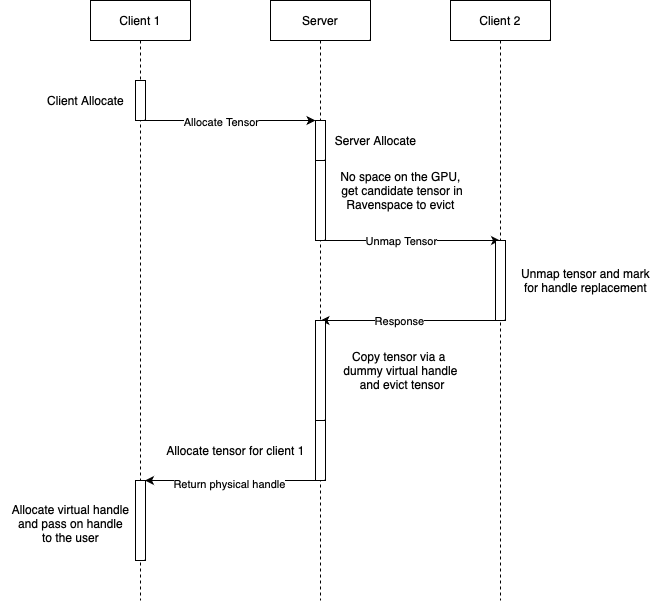
\includegraphics[height=8cm, width=8cm]{figures/Offloading.drawio.png}
	\caption{Sequence Diagram for Offloading}
\end{figure}
\FloatBarrier


\section{Implementation}

\section{Evaluation and Benchmarks}

\section{Future Work}
\subsection{Multi GPU Design}

\section{Conclusion}


\bibliographystyle{unsrtnat}
\bibliography{references}  %%% Uncomment this line and comment out the ``thebibliography'' section below to use the external .bib file (using bibtex) .


%%% Uncomment this section and comment out the \bibliography{references} line above to use inline references.
% \begin{thebibliography}{1}

% 	\bibitem{kour2014real}
% 	George Kour and Raid Saabne.
% 	\newblock Real-time segmentation of on-line handwritten arabic script.
% 	\newblock In {\em Frontiers in Handwriting Recognition (ICFHR), 2014 14th
% 			International Conference on}, pages 417--422. IEEE, 2014.

% 	\bibitem{kour2014fast}
% 	George Kour and Raid Saabne.
% 	\newblock Fast classification of handwritten on-line arabic characters.
% 	\newblock In {\em Soft Computing and Pattern Recognition (SoCPaR), 2014 6th
% 			International Conference of}, pages 312--318. IEEE, 2014.

% 	\bibitem{keshet2016prediction}
% 	Keshet, Renato, Alina Maor, and George Kour.
% 	\newblock Prediction-Based, Prioritized Market-Share Insight Extraction.
% 	\newblock In {\em Advanced Data Mining and Applications (ADMA), 2016 12th International 
%                       Conference of}, pages 81--94,2016.

% \end{thebibliography}


\end{document}
